\documentclass[12pt]{article}
\usepackage[margin=1in]{geometry}
\usepackage{tabularx}
\usepackage{enumerate}
\usepackage{amsmath}
\usepackage{graphicx}
\usepackage{placeins}
\usepackage[hidelinks=true]{hyperref}
\renewcommand{\labelitemi}{$ $}
\renewcommand{\labelitemii}{$\bullet$}
\renewcommand{\labelitemiii}{$\circ$}
\renewcommand{\labelitemiv}{$\diamond$}
\newcommand{\requirement}[4] {
		\noindent
		\begin{center}\textbf{Requirement\\}\textit{#1}\\\end{center}
		\textbf{Description:} #2\\
		\textbf{User Story:} ``#3''\\
		\textbf{User Case Diagram:} #4\\
}

\title{
	\huge Requirements Document\\
	\large ASU Capstone Portal\\
	\small Version No. 1.0\\
	\small Last Modified: April 24, 2016
}

\author{
	Team Members: Ryan Simmons, Brett Hansen
}
\date{}
\begin{document}

\begin{titlepage}

\null
\nointerlineskip
\vfill
\let\snewpage \newpage
\let\newpage \relax
\maketitle
\let \newpage \snewpage
\vfill 
\break

\end{titlepage}

\null
\nointerlineskip
\vfill
\let\snewpage \newpage
\let\newpage \relax
\tableofcontents{}
\let \newpage \snewpage
\vfill 
\break

\section{Revision History}

\begin{center}
\begin{tabularx}{\linewidth}{ |c|c|X|X| }
	\hline
	\textbf{Revision} & \textbf{Date} & \textbf{Authors} & \textbf{Remarks} \\
	\hline\hline
	1.0 & 4-28-16 & Ryan Simmons, Brett Hansen & Initial Draft \\
	\hline
\end{tabularx}
\end{center}

\section{Introduction}
Currently, managing the projects for the CS/CSE capstones is a completely manual process, where proposals by faculty or companies are sent as word or pdf files to the university. Then students download a zip file of all the projects and an excel file listing basic demographic information of the projects. Students then submit their preferred projects and teammates, and the instructors of the course choose how to best allocate projects and teams.

\subsection{Purpose}

The purpose of the ASU Capstone Portal is to provide an easy to use, centralized system that allows students, sponsors, and instructors to participate in the ASU Capstone process, and make the experience more intuitive, more efficient, and more organized for all parties involved.

\subsection{Scope}

Through three separate subsystems, The ASU Capstone Portal will allow students, sponsors, and instructors to access a personalized portal used to complete various tasks for the Capstone course. Sponsors will be able to submit proposals though a simple web form and see the status of their submitted proposals, students will have tools to aid in the process of project and team selection, and instructors will have the ability to manage the process from beginning to end with greater organization and control.

\section{Product Overview}

The project will involve building an online portal to handle all of these tasks in one simple interface. Faculty and companies can submit proposals in the online portal through web forms (possibly using Google Docs). Instructors will be able to look through these proposals and select which are viable, then publish them to the students. Students will be easily able to look through all the projects and rank them according to their preferences, as well as choose their preferred teammates. An algorithm can then choose how to best allocate projects and teams and allow the instructors control to change selections.

\subsection{Product Users}

The product will accommodate 3 primary users, each with a separate branch of access and feature set. The users include a student enrolled in the ASU capstone course, the instructor of said course, and a project sponsor, which can either be an outside organization or an ASU faculty member.

\subsection{Use Case Actors}

The following table describes the actors of the system. An ``actor'' may be generally described as a functional role of a user of the system.

\begin{center}
\begin{tabularx}{\linewidth}{ |r|X| }
	\hline
	\textbf{Actor} & \textbf{Description} \\
	\hline\hline
	Sponsor & An organization or faculty member proposes and then oversees a capstone project. \\
	\hline
	Student & Students in the capstone course work in teams to complete projects proposed by the sponsors. \\
	\hline
	Instructor & The instructor of the capstone course has control over how project proposals, student teaming, and project-team matching is done. \\
	\hline
\end{tabularx}
\end{center}

\subsection{Goals}

The following list describes the primary system goals for each of the actors:

\begin{itemize}
	\item \textbf{Student}
	\begin{itemize}
		\item Register within the system as a student
		\item Create small profile detailing major and topics of interest
		\item Team management
		\begin{itemize}
			\item Create new team
			\begin{itemize}
				\item Private or public
			\end{itemize}
			\item View existing teams
			\item Join public teams
		\end{itemize}
		\item Project management
		\begin{itemize}
			\item View all projects approved for the current semester
			\item Rate each project according to personal preference
		\end{itemize}
		\item Student management
		\begin{itemize}
			\item View other students in the class
			\begin{itemize}
				\item Major, interests, schedule team info
			\end{itemize}
		\end{itemize}
	\end{itemize}

	\item \textbf{Sponsor}
	\begin{itemize}
		\item Register within the system as a student
		\item Create small profile detailing description of organization
		\item Submit project proposals
		\item View status of submitted proposals
	\end{itemize}

	\item \textbf{Instructor}
	\begin{itemize}
		\item Sponsor Interaction
		\begin{itemize}
			\item View submitted proposals
			\item Approve/Deny proposals
			\item Request additional info
		\end{itemize}
		\item Team management
		\begin{itemize}
			\item View teams
			\item Edit teams
		\end{itemize}
		\item Settings
		\begin{itemize}
			\item Modify proposal form
			\item Allow/disallow student team selection
			\item Allow/disallow student project selection
		\end{itemize}
	\end{itemize}
\end{itemize}

\section{Assumptions and Dependencies}
Users of the portal must be connected to the internet to use the system.
Student users will need to be currently enrolled in a current capstone course to register for the system.

\section{High-level Subsystem Requirements}
The system will have three major subsystems: the student system, the sponsor system, and the instructor system. Each subsystem will be tailored to the respective user group. Upon accessing the system, all users, regardless of role, will interact with the log in system. Students and sponsors will register if they have not previously done so, whereas instructors will be given manual access. If registered, users will be prompted to log in with their credentials. Each subsytem will have separate features based on the role of the user, though many of these components will overlap information between the separate subsytems. All information will be stored in a single database, allowing information to be served dynamically to each user based on their role.
\begin{figure}[!htb]
	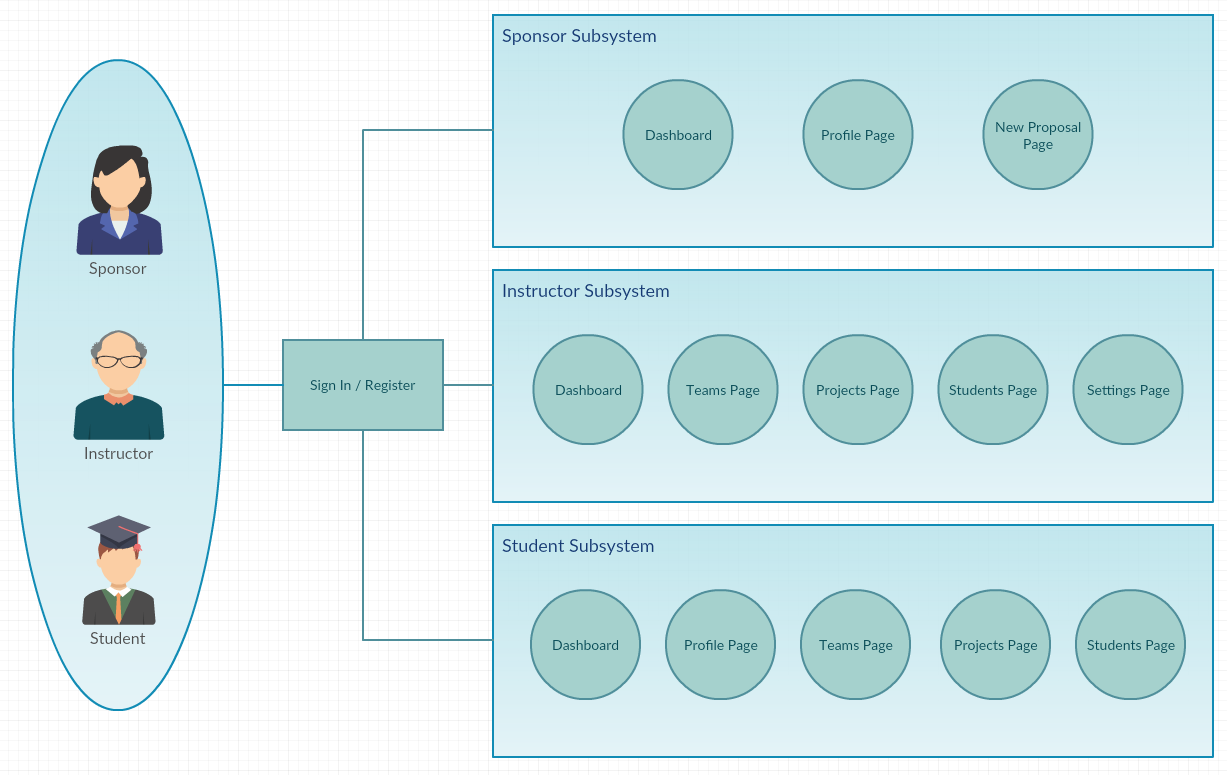
\includegraphics[width=\linewidth]{subsystems.png}
	\caption{Diagram of subsystems.}
	\label{fig:subsystems}
\end{figure}

\FloatBarrier
\subsection{Sponsor Framework}

\subsubsection{Description}

The sponsor framework portion of the portal will allow prospective and current sponsors to propose and manage projects for students to complete. In addition to these functions, sponsors will also be able to provide a brief description as well as demographics for their organization so that students can make more informed choices about their preferred projects.

\subsubsection{Requirements}
\requirement{Register within the system as a sponsor}
			{A prospective sponsor will have the ability to register with the system. They must have the ability to create a small yet descriptive profile indicating the type of organization, as well as a brief overview of the organization.}
			{As a sponsor, I want be able to easily register with the capstone portal, giving a brief description of my organization, so that I may submit my proposal idea for review and have students learn more about my organization.}
			{\autoref{fig:sponsor}}

\requirement{Create and submit project proposals}
			{An organization must be able to create new project proposals by filling out a provided online form, as well as submit the form to the school for review from the portal.}
			{As a sponsor, I want to have the ability to submit a project proposal to the school through an easy to use online form, so that I can quickly complete the task and make better use of my time.}
			{\autoref{fig:sponsor}}

\requirement{Modify proposals if requested by instructor}
			{Once a proposal has been submitted, it will be sent to the school for review and appear in the sponsors dashboard with a status of pending. If more information or changes are needed by the school, the proposal will be marked as such, and sponsors should have the ability to edit the submitted proposal as requested.}
			{As a sponsor, I want to see the status of my proposal from my dashboard in real time, so that I will know if my proposal is accepted or not, and should it need to be modified, I want the ability to make changes to my submitted proposal and resubmit.}
			{\autoref{fig:sponsor}}

\subsubsection{Use Case Diagram}
\begin{figure}[!htb]
	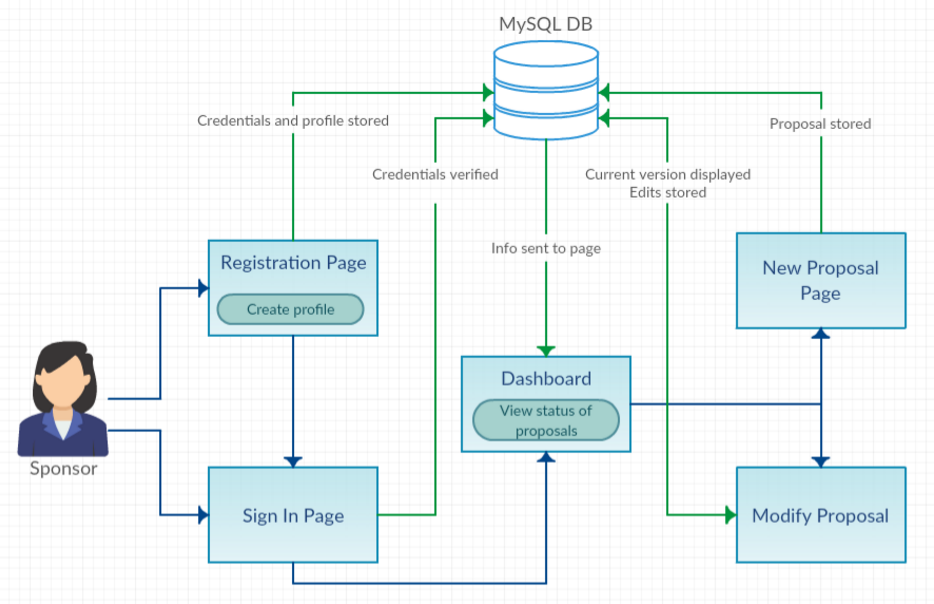
\includegraphics[width=\linewidth]{sponsor.png}
	\caption{User case diagram illustrating all requirements for sponsors.}
	\label{fig:sponsor}
\end{figure}

\subsection{Student Framework}

\subsubsection{Description}

Students will use the portal initially to review the proposed projects for the current semester. In addition to being able to review these proposed projects and rank them according to preference, students can view the profiles of sponsors to further judge their preference of a project.

To facilitate more informed teammaking, students will have the ability to describe their interests and fields, as well as their schedules and time availability. From this information students can make teams with their classmates, or the instructor will form the teams, depending on the instructor’s preferences.
Once teams are created, students can analyze which projects best fit their teams and a project proposal will be assigned to their team based on their compatibility with the project and the instructor’s preferences.

\subsubsection{Requirements}

\requirement{Register within the system as a student}
			{A student will have the ability to register with the system. They must have the ability to create a small yet descriptive profile indicating their major, as well as a brief list of there strengths/interests.}
			{As a student, I want to be able to easily register for the system and give my basic profile information, including interests, so that I am able to begin viewing other students, their interests, and the approved projects.}
			{\autoref{fig:student}}

\requirement{Create a new team or join an existing one}
			{Student will have the ability to create a new team, with the option of making it public or private. A public team would allow other students to join immediately, whereas a private team would allow other students to request access. If the student does not wish to create a new team, they can view the existing ones and join/request access.}
			{As a student, I want to have the choice of browsing the existing teams and choosing one to join, or creating my own either public or private team from scratch, so that I can have greater control and flexibility in the team making process.}
			{\autoref{fig:student}}

\requirement{View and rate all projects approved for the current semester}
			{Students will have the ability to view all approved projects, read a short description of each, and access each projects proposal for more specific information. They will also have the ability to rate each project according to their personal preferences.}
			{As a student, I want to be able to see all of the approved projects in a single, well organized interface, displayed in a way that allows me to easily rate each project, so that I can sort through the projects more efficiently, make better selections, and provide a wider scope of preferences to my instructor, allowing for a more fair distribution of projects.}
			{\autoref{fig:student}}

\requirement{View other students in the class}
			{Students will have the ability to view all of the other students in the class as well as see the major, interests, and current team info for each student.}
			{As a student, I want to be able to easily view the other students in the course and see details about each person, including the major and interests, so that I can learn more about my peers and make a better choice when forming a team.}
			{\autoref{fig:student}}

\subsubsection{Use Case Diagram}
\begin{figure}[!htb]
	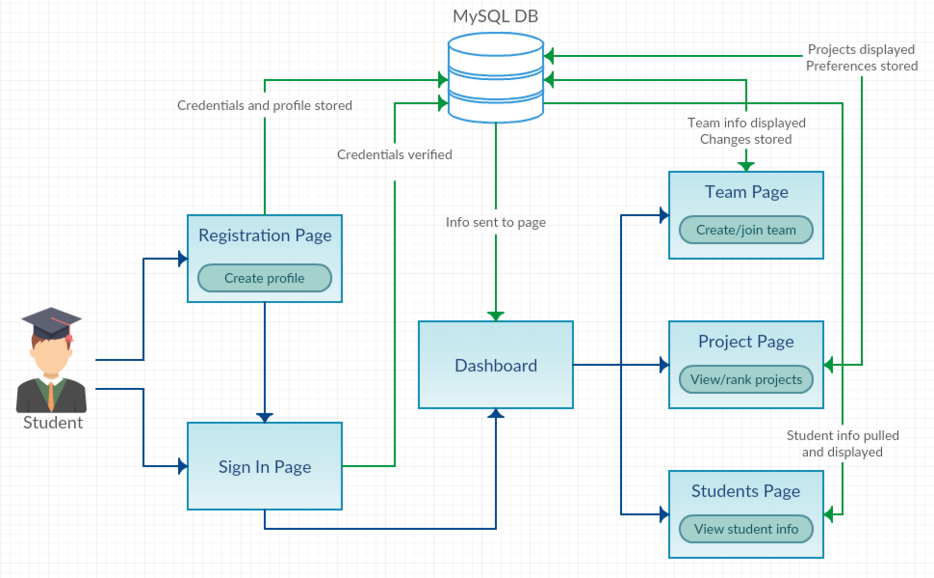
\includegraphics[width=\linewidth]{student.png}
	\caption{User case diagram illustrating all requirements for students.}
	\label{fig:student}
\end{figure}

\subsection{Instructor Framework}

\subsubsection{Description}

Instructors need to be able to manage classes of students as well as the group of sponsors and their project proposals. Instructors also have the ability to allow and disallow certain features such as student teammaking. Instructors can edit the project proposal form to best fit their class’ projects.

\subsubsection{Requirements}

\requirement{Manage all proposal submissions}
			{An instructor will be able to review all proposals that have been submitted and approve/reject them from the system. If a proposal is missing information, or the instructor feels modifications must be made, they have the ability to mark the proposal as such, giving an explanation as to what is needed. }
			{As an instructor, I want to view all of the proposals that have been submitted from within a single, well organized interface, so that I can easily approve them, reject them, or send them back to the sponsor requesting more information.}
			{\autoref{fig:instructor}}

\requirement{Manual management of teams}
			{An instructor will be able to view all teams formed by the students, as well as modify them however they choose - i.e. moving a student from one team to another.}
			{As an instructor, I want to have to ability to not only view the teams formed by the students, but also the ability to manual move students from one to another, or manually assign students to a team, so that I can better control the placement of students if necessary.}
			{\autoref{fig:instructor}}

\requirement{Modify default functionality how they see fit}
			{An instructor will be able to override much of the default functionality if they choose, to better tailor the system to their preferences. This includes the ability to modify the content of the proposal form, allow or disallow student team selection, as well as manually create teams or assign projects.}
			{As an instructor, I want the ability to easily modify the default functionality of the system, including the proposal form that sponsors use, and have option to either allow or disable certain student features such as team selection and project selection, so that I can have greater control in how the course is ran.}
			{\autoref{fig:instructor}}

\subsubsection{Use Case Diagram}
\begin{figure}[!htb]
	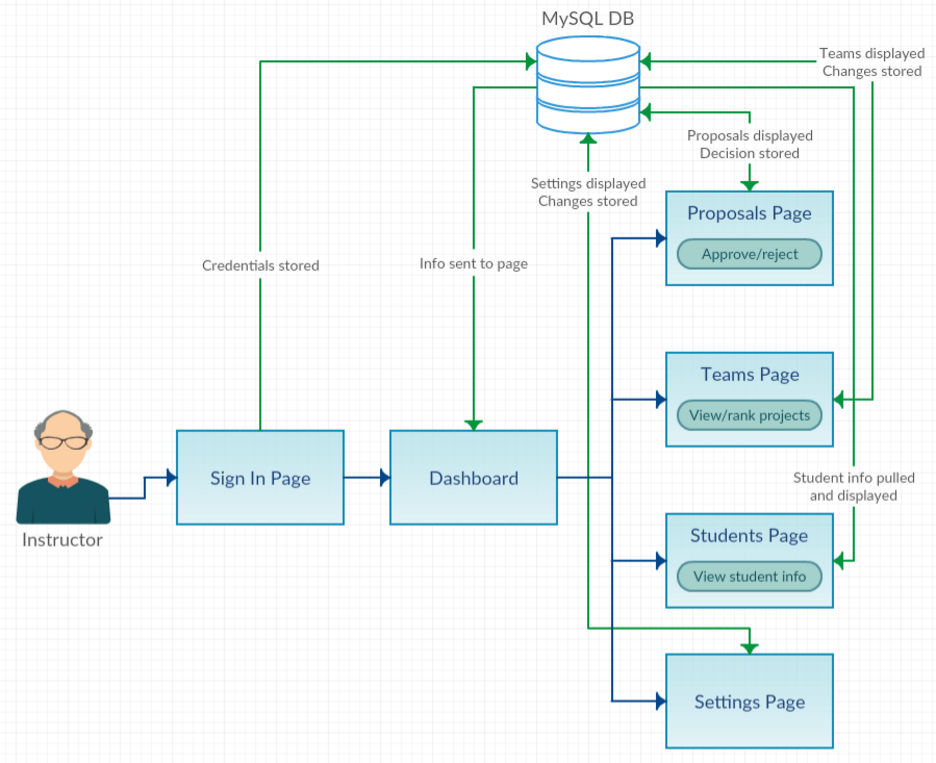
\includegraphics[width=\linewidth]{instructor.png}
	\caption{Use case diagram illustrating all requirements for instructors.}
	\label{fig:instructor}
\end{figure}

\section{System Requirements}

\subsection{Platform Support}

Because the portal is entirely web-based, it will not be platform dependent. All platforms with a modern browser that is web connected will be able to access the portal, including mobile platforms.

\subsection{Database Support}

The portal will be supported by a single MySQL database where information on users, proposals, teams, and instructor preferences will be stored and queried on demand.

\subsection{Browser Support}
The portal will be supported by all modern browsers (Chrome, Firefox, IE8+, Safari, etc.) and utilize bootstrap, a mobile-first UI platform, to ensure functionality and consistency across all platforms.

\section{Application Requirements}

\subsection{Security}
Sponsors will be free to make an account and submit proposals without previously having credentials or authorization to do so. However, the only information accessible to sponsors before their proposals are approved will be information they provide for a project proposal. Sponsors will not be able to view each other's projects, nor will any visitor to the site without proper credentials.

All other parts of the system will not be publicly accessible. Only instructors and those users added to the system by instructors (namely students) will be able to view all project proposals, teams, and student profiles.

Login information will never be stored in plain text. When a new account is made and a password is chosen, the password will be concatenated with a salt and then hashed before being stored (alongside the generated salt) in the database. In this way, user passwords are never recoverable into their unhashed form and the system will be defended against dictionary attacks on users. Commonly employed credential protection techniques, such as a maximum number of password guesses and secure password resets will be employed.

\subsection{Localization}

The portal will only have support in English and is intended for users in the Arizona timezone (UTC -7), however, features will not be explicitly restricted by locale or timezone.

\subsection{Installation Requirements}

The client computer or mobile device used to access the portal needs only to have a modern browser installed to use the system.

\end{document}